%Handouts
\documentclass[handout]{beamer}
\mode<presentation> {%
	\usetheme[]{Boadilla}
	\usecolortheme{orchid}
	\setbeamercovered{transparent}
	\setbeamersize{text margin left=0.7cm}
  \setbeamersize{text margin right=0.7cm}
  \setbeamertemplate{enumerate item}[square]
  \setbeamertemplate{enumerate subitem}[circle]
  \setbeamertemplate{enumerate subsubitem}[>]
  \setbeamertemplate{itemize item}[square]
  \setbeamertemplate{itemize subitem}[circle]
  \setbeamertemplate{itemize subsubitem}[>]
}

\usepackage{pstricks}
\usepackage{pst-node}
\usepackage{bm}
\usepackage[utf8]{inputenc}
\usepackage[spanish]{babel}
\usepackage{times}
\usepackage[T1]{fontenc}
\usepackage{graphicx}
\usepackage{multirow}
\usepackage{pifont}
\usepackage{rotating}
\usepackage{colortbl}
\usepackage[framed]{mcode}
\usepackage{verbatim}
\usepackage{textcomp}
\lstset{literate=
  {á}{{\'a}}1 {é}{{\'e}}1 {í}{{\'i}}1 {ó}{{\'o}}1 {ú}{{\'u}}1
  {Á}{{\'A}}1 {É}{{\'E}}1 {Í}{{\'I}}1 {Ó}{{\'O}}1 {Ú}{{\'U}}1
  {à}{{\`a}}1 {è}{{\`e}}1 {ì}{{\`i}}1 {ò}{{\`o}}1 {ù}{{\`u}}1
  {À}{{\`A}}1 {È}{{\'E}}1 {Ì}{{\`I}}1 {Ò}{{\`O}}1 {Ù}{{\`U}}1
  {ä}{{\"a}}1 {ë}{{\"e}}1 {ï}{{\"i}}1 {ö}{{\"o}}1 {ü}{{\"u}}1
  {Ä}{{\"A}}1 {Ë}{{\"E}}1 {Ï}{{\"I}}1 {Ö}{{\"O}}1 {Ü}{{\"U}}1
  {â}{{\^a}}1 {ê}{{\^e}}1 {î}{{\^i}}1 {ô}{{\^o}}1 {û}{{\^u}}1
  {Â}{{\^A}}1 {Ê}{{\^E}}1 {Î}{{\^I}}1 {Ô}{{\^O}}1 {Û}{{\^U}}1
  {Ã}{{\~A}}1 {ã}{{\~a}}1 {Õ}{{\~O}}1 {õ}{{\~o}}1
  {œ}{{\oe}}1 {Œ}{{\OE}}1 {æ}{{\ae}}1 {Æ}{{\AE}}1 {ß}{{\ss}}1
  {ű}{{\H{u}}}1 {Ű}{{\H{U}}}1 {ő}{{\H{o}}}1 {Ő}{{\H{O}}}1
  {ç}{{\c c}}1 {Ç}{{\c C}}1 {ø}{{\o}}1 {å}{{\r a}}1 {Å}{{\r A}}1
  {€}{{\euro}}1 {£}{{\pounds}}1 {«}{{\guillemotleft}}1
  {»}{{\guillemotright}}1 {ñ}{{\~n}}1 {Ñ}{{\~N}}1 {¿}{{?`}}1
}

\definecolor{olivegreen}{rgb}{0.0,0.5,0.0}
\definecolor{general}{rgb}{0.9 0.9 1}%
\newrgbcolor{colorsistema}{0 1 1}
\newrgbcolor{colorviolet}{0.9 0.8 1}

\title[Procesamiento de Señales]{Procesamiento de imágenes}
\author[Jesús Chacón Sombría]{%[Author, Another] % (optional, use only with lots of authors)
\textit{Ingeniería Electrónica de Comunicaciones }\\
\vspace{0.6cm}
\small Jesús Chacón Sombría}%\inst{1} \and S.~Another\inst{2}}
% - Use the \inst{?} command only if the authors have different
%   affiliation.

\institute[DACYA. UCM] % (optional, but mostly needed)
{
\footnotesize  Departamento de Arquitectura de Computadores y Automática.\\
  Universidad Complutense de Madrid
}

\date[Procesamiento de imágenes] % (optional)
{\footnotesize Curso 2024-2025}%{\today / Master}
\subject{Talks}

\pgfdeclareimage[height=0.75cm]{logo}{ucm.png}

\usepackage[absolute,overlay]{textpos}
\setlength{\TPHorizModule}{1mm}
\setlength{\TPVertModule}{1mm}
\newcommand{\MyLogo}{%
\begin{textblock}{14}(116.0,0.6)
  \pgfuseimage{logo}
\end{textblock}
}

\makeatletter
\numberwithin{section}{part}
\AtBeginPart{
\beamer@tocsectionnumber=0\relax
\frame{\partpage}
}
\makeatother

\begin{document}

\begin{frame}
  \titlepage
\end{frame}

\newcommand*\oldmacro{}%
\let\oldmacro\insertshorttitle%
\renewcommand*\insertshorttitle{%
 %\MyLogo
  \oldmacro\hfill%
}

\AtBeginSection[]
{
  \begin{frame}%<beamer>
    \frametitle{Esquema}
  \small
    \tableofcontents[sectionstyle=show/shaded,subsectionstyle=show/shaded/hide]
  \end{frame}
}

\AtBeginSubsection[]
{
  \begin{frame}%<beamer>
    \frametitle{Esquema}
    \small
   \tableofcontents[sectionstyle=show/shaded,subsectionstyle=show/shaded/hide]
      \end{frame}
}



%%%%%%%%%%%%%%Empieza la presentacion%%%%%%%%%%%%%%%%%%%%%%%%%%%%%%%%%%%%

%\begin{frame}
%\frametitle{Esquema}
 %   \tableofcontents
%\end{frame}

\section{Objetivos}

\begin{frame}
\frametitle{Objetivos del tema}

 Introducci\'{o}n de otras técnicas  de procesamiento de se\~{n}ales digitales:


\vspace{0.2cm}

\begin{itemize}
\normalsize
\visible<2->{
\item Procesamiento de im\'{a}genes digitales:

\vspace{0.1cm}

\begin{itemize}

\item Transformada de Fourier Discreta 2D

\vspace{0.1cm}

\item Filtros FIR

\vspace{0.1cm}

\item Transformaciones basadas en histograma
\end{itemize}
}

\vspace{0.1cm}

% \visible<3->{
% \item An\'{a}lisis de se\~{n}ales no estacionarias:

% \vspace{0.1cm}

% \begin{itemize}

% \item Transformada de Fourier de corta duraci\'{o}n: espectrograma

% \vspace{0.1cm}

% \item Wavelets
% \end{itemize}
% }

\end{itemize}

\end{frame}


\section{Introducciónn al procesamiento de imagenes digitales}
  \begin{frame}\frametitle{Visi\'{o}n por computador}
    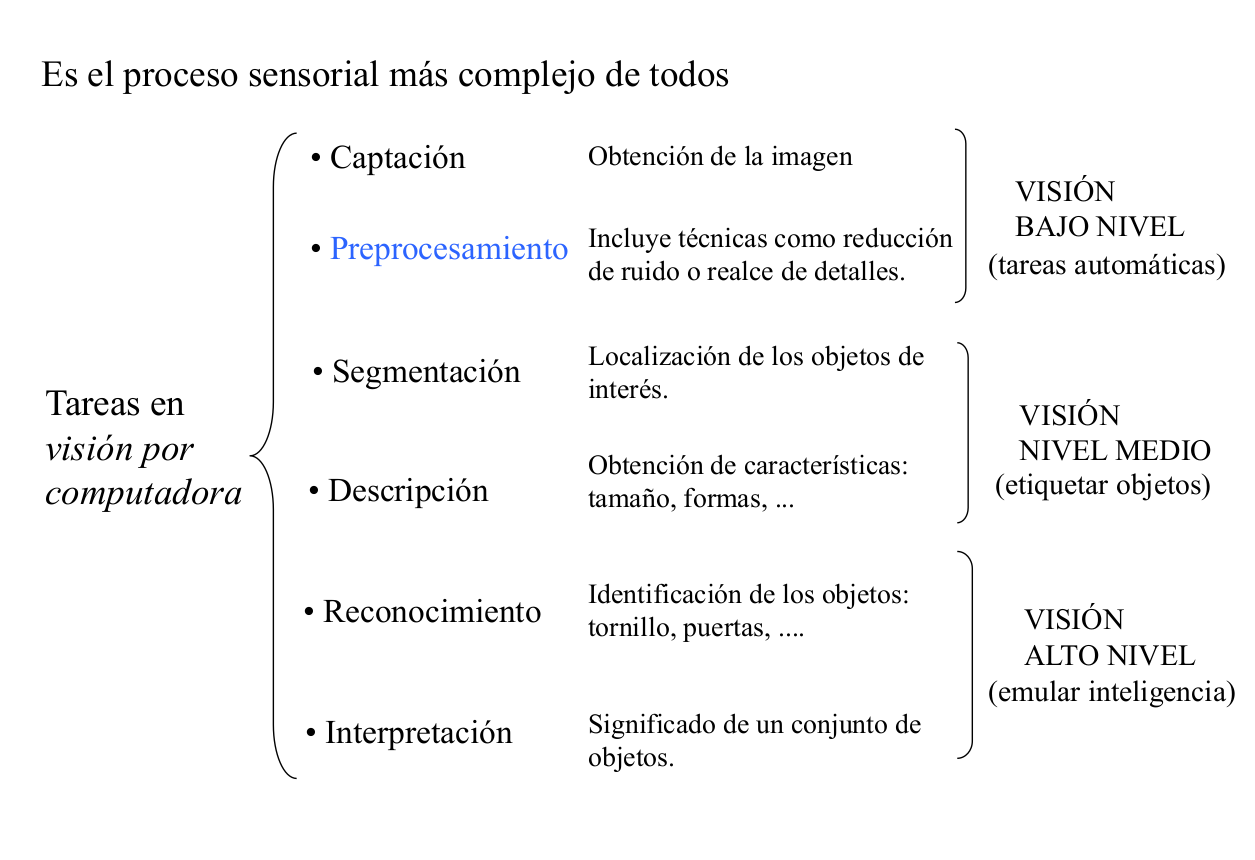
\includegraphics[width=10cm]{Figures/Clasificacion.png}
  \end{frame}

\subsection{Adquisición y repesentación de imágenes}

\begin{frame}
  \frametitle{Adquisición de imágenes}
  Las imágenes provienen de diferentes fuentes y se digitalizan a través de diferentes medios.
  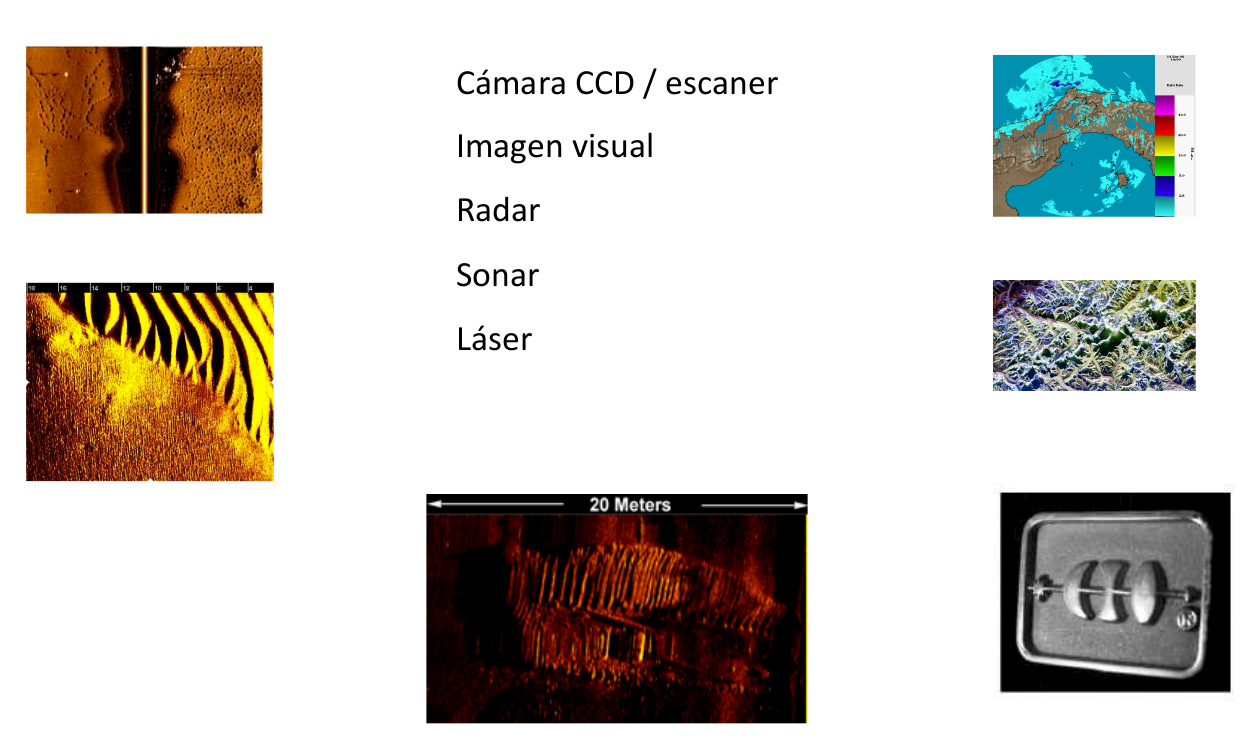
\includegraphics[width=10cm]{./Figures/AdquisicionImagenes}
\end{frame}

\begin{frame}
  \frametitle{Representación de imágenes en el computador}
  \small
  Una imagen es una señal bidimensional $(x,y)$ con uno o varios canales:\\
  \vspace{-0.1cm}
  \begin{itemize}
    \small
    \item \textbf{Imagen de intensidad (B/N) o de escala de grises}: en cada pixel (posici\'{o}n de la matriz de valores) se almacena un \'{u}nico valor que representa la intensidad luminosa en el punto correspondiente.\\
    \vspace{-0.2cm}
    \begin{columns}[t]
      \hspace{1cm}\begin{column}{1.8cm}
        
        \includegraphics[width=1.7cm,trim={0cm 0cm 0cm 0cm},clip,angle=0]{./Figures/Moon.eps}\\
      \end{column}
      \hspace{-0.5cm}\begin{column}{8cm}
      \footnotesize\\
      Es una matriz de MxN valores:
      \vspace{-0.15cm}
      \begin{itemize}
        \scriptsize
        \item uint8 (0-255)
        \vspace{-0.15cm}
        \item uint16 (0-65535)
        \vspace{-0.15cm}
        \item double (0.0-1.0)
        \vspace{-0.15cm}
        \item binario (0,1)
      \end{itemize}
      En cualquier caso:
      (0,max) $\rightarrow$ (negro,maximo)
      \end{column}
  \end{columns}

  \item \textbf{Imagen de color verdadero (RGB)}: se almacenan 3 valores por pixel, que representan su proporcion de rojo, verde y azul.
  \begin{columns}[t]
    \hspace{0.2cm}\begin{column}{1.8cm}

      \includegraphics[width=1.7cm,trim={0cm 0cm 0cm 0cm},clip,angle=0]{./Figures/Foot.eps}
    \end{column}
    \hspace{-0.9cm}\begin{column}{2.5cm}
      \footnotesize      
      Es una matriz de MxNx3 valores, con los rangos y tipos anteriores.
    \end{column}
    \hspace{-0.9cm}  \begin{column}{1.8cm}

      \includegraphics[width=1.7cm,trim={0cm 0cm 0cm 0cm},clip,angle=0]{./Figures/FootR.eps}
    \end{column}
    \hspace{-0.7cm}\begin{column}{1.8cm}

      \includegraphics[width=1.7cm,trim={0cm 0cm 0cm 0cm},clip,angle=0]{./Figures/FootG.eps}
    \end{column}
    \hspace{-0.7cm}\begin{column}{1.8cm}

      \includegraphics[width=1.7cm,trim={0cm 0cm 0cm 0cm},clip,angle=0]{./Figures/FootB.eps}
    \end{column}
  \end{columns}
  \item  \textbf{Imagen de color LAB}: se almacenan 3 valores por pixel: intensidad, porcentaje rojo-verde, azul-amarillo.
  \end{itemize}
\end{frame}

\begin{frame}
  \frametitle{Representación de imágenes en el disco}
  \small
  Las imágenes se pueden almacenar en disco en diferentes formatos:

  \begin{itemize}
    \item \textbf{Raw}: se almacena directamente la matriz de valores de intensidad.
    \item \textbf{Formatos comprimidos sin perdida de información} (ej: \emph{tiff}): 
    reducen el tamaño eliminando redundancias, pero sin provocar pérdida de información.
  
    \item \textbf{Formatos comprimidos con perdida de información} (ej: \emph{jpg}): 
    (ej: \emph{tiff}): 
    reducen el tamaño a costa de perder parte de la información de la imágen.
  \end{itemize}
\end{frame}


\begin{frame}
  \frametitle{Carga y dibujo de im\'{a}genes con Matlab}
  \small

  Funciones de Matlab:

  \begin{itemize}

  \small

  \item Cargar im\'{a}genes: \color{blue} im=imread(\textit{NombreFichero}) \color{black}

  \color{gray}
  La funci\'{o}n carga im\'{a}genes almacenadas en ficheros de diferentes formatos y crea la matriz correspondiente.
  \color{black}

  \item Crear una imagen sint\'{e}tica en el formato adecuado:
  \begin{itemize}
  \item Cualquiera de las ordenes habituales de Matlab
  \item \color{blue} uint8, uint16, double \color{black}
  \end{itemize}

  \item Representar una imagen: \color{blue} imshow\color{black}

  \hspace{0.5cm}\color{blue} imshow(im) \color{black}

  \hspace{0.5cm}\color{blue} imshow(im,[minx,max]) \color{black}

  \hspace{0.5cm}\color{blue} imshow(255*im/max(im(:)),colormap(\textit{NombreColorMap})) \color{black}

  \color{gray}
  En el segundo caso se re-escala la imagen para mostrar los valores entre los limites. En el segundo, se elige un mapa de colores para lograr una representaci\'{o}n m\'{a}s comprensible.

  \color{black}
  \end{itemize}
\end{frame}



\begin{frame}
\frametitle{Ejemplos de carga/dibujo de im\'{a}genes I}



\begin{columns}[t]
\begin{column}{7cm}

\color{olivegreen}Ejemplo: \color{black} Imagen B/N

\vspace{-0.5cm}

\lstinputlisting{./Matlab/Imagen1.m}

\scriptsize
\color{gray}{>> im  \hspace{1cm}      537x358 \hspace{1cm}    uint8}

\end{column}

\hspace{-0.4cm} \begin{column}{1.8cm}

\fbox{\includegraphics[width=1.7cm,trim={0cm 0cm 0cm 0cm},clip,angle=0]{./Figures/Moon1.eps} }

\vspace{0.1cm}
\scriptsize Imagen 1 y 3

\end{column}

\hspace{-0.4cm} \begin{column}{1.8cm}

\fbox{
\includegraphics[width=1.7cm,trim={0cm 0cm 0cm 0cm},clip,angle=0]{./Figures/Moon2.eps} }

\vspace{0.1cm}
\scriptsize Imagen 2

\end{column}

\end{columns}

%%%%%%%

\visible<2->{

\begin{columns}[t]
\begin{column}{7cm}

\color{olivegreen}Ejemplo: \color{black} Imagen Color

\vspace{-0.5cm}

\lstinputlisting{./Matlab/Imagen2.m}


\scriptsize
\color{gray}{>> im  \hspace{1cm}      256x320x3  \hspace{1cm}    uint8}



\end{column}

\hspace{-0.4cm} \begin{column}{1.8cm}

\vspace{1.0cm}

\includegraphics[width=1.7cm,trim={0cm 0cm 0cm 0cm},clip,angle=0]{./Figures/Foot.eps}

\vspace{0.1cm}
\scriptsize Imagen RGC

\end{column}

\hspace{-0.4cm} \begin{column}{1.8cm}

\vspace{1.0cm}

\includegraphics[width=1.7cm,trim={0cm 0cm 0cm 0cm},clip,angle=0]{./Figures/FootR.eps}

\vspace{0.1cm}
\scriptsize Canal red

\end{column}


\end{columns}

}


\end{frame}


\begin{frame}
\frametitle{Ejemplos de carga/dibujo de im\'{a}genes I}




\begin{columns}[t]
\begin{column}{7cm}

\color{olivegreen}Ejemplo: \color{black} Generaci\'{o}n de im\'{a}genes

\vspace{-0.5cm}

\lstinputlisting{./Matlab/Imagen3.m}


\end{column}

\hspace{-0.4cm} \begin{column}{1.8cm}

\vspace{1.0cm}

\includegraphics[width=1.7cm,trim={0cm 0cm 0cm 0cm},clip,angle=0]{./Figures/ImSintetica1.eps}

\vspace{0.1cm}
\scriptsize Imagen 1

\end{column}

\hspace{-0.4cm} \begin{column}{1.8cm}

\vspace{1.0cm}

\includegraphics[width=1.7cm,trim={0cm 0cm 0cm 0cm},clip,angle=0]{./Figures/ImSintetica2.eps}

\vspace{0.1cm}
\scriptsize Imagen 2

\end{column}


\end{columns}


\vspace{0.3cm}
%%%%%%

\visible<2->{

\begin{columns}[t]
\begin{column}{5.4cm}

\color{olivegreen}Ejemplo: \color{black} Usar mapa de colores

\vspace{-0.5cm}

\lstinputlisting{./Matlab/Imagen4.m}


\end{column}

\hspace{-0.6cm} \begin{column}{1.8cm}



\includegraphics[width=1.7cm,trim={0cm 0cm 0cm 0cm},clip,angle=0]{./Figures/Colormap1.eps}

\vspace{0.1cm}
\scriptsize Imagen 1

\end{column}

\hspace{-0.8cm} \begin{column}{1.8cm}



\includegraphics[width=1.7cm,trim={0cm 0cm 0cm 0cm},clip,angle=0]{./Figures/Colormap2.eps}

\vspace{0.1cm}
\scriptsize Imagen 2

\end{column}

\hspace{-0.8cm} \begin{column}{1.8cm}



\includegraphics[width=1.7cm,trim={0cm 0cm 0cm 0cm},clip,angle=0]{./Figures/Colormap3.eps}

\vspace{0.1cm}
\scriptsize Imagen 3

\end{column}


\end{columns}}

\end{frame}


\subsection{Transformada de Fourier Discreta 2D}

\begin{frame}
\frametitle{Introducci\'{o}n Transformada de Fourier 2D}

\small

En el caso de las se\~{n}ales 1D (que hemos representado habitualmente frente al tiempo) hemos visto 3 Transformadas de Fourier diferentes:
\begin{itemize}

\item Transformada de Fourier continua ($x(t) \rightarrow X(jw)$). Se utiliza para se\~{n}ales continuas y obtiene transformadas en frecuencias continuas

\item Transformada de Fourier en tiempo discreto ($x(n) \rightarrow X(e^{jw})$). Se utiliza para se\~{n}ales discretas y obtiene transformadas en frecuencias continuas.

\item Transformada de Fourier discreta (FFT, $x(n) \rightarrow X(k)$). Se utiliza para se\~{n}ales discretas y obtiene transformadas en frecuencias discretas.

\end{itemize}

\visible<2->{
Como la \'{u}ltima es la que se puede computar facilmente con un ordenador y se relaciona con las anteriores (represent\'{a}ndola ante $w_d=2 \pi*[0:N-1]/N$ \'{o} $w_c=w_d*F_s$), vamos a ver directamente la
Transformada de Fourier Discreta (FFT) para im\'{a}genes digitales. }

\vspace{0.1cm}

\visible<3->{
Antes de proceder, hay que tener en cuenta que:

\vspace{-0.7cm}

\begin{columns}[t]

\begin{column}{6cm}

\begin{itemize}
\item $u=sen(w_c*t)$ y  $w_c=\frac{2\pi}{T}$ rad/s

\vspace{-0.2cm}

\item $u=sen(w_c*x)$ y $w_c= \frac{2\pi}{T}$ rad/m
\end{itemize}

\end{column}

\visible<4->{
\begin{column}{3cm}

\begin{itemize}


\item $t=n \cdot T_s$

\vspace{-0.2cm}

\item $x= n \cdot D_x$\end{itemize}

\end{column}}


\end{columns}

}

\end{frame}


\begin{frame}
\frametitle{Definici\'{o}n de la Transformada de Fourier Discreta 2D }

\small

Definiciones para se\~{n}ales 1D f(n) de longitud N:

\vspace{0.1cm}


\begin{itemize}

\item  $X(k)=DFT(x(n))=\sum_{n=0}^{N-1} x(n) e^{- j \frac{2 \pi  k}{N} n}=\sum_{n=0}^{N-1} x(n) e^{-2\pi j \frac{ kn}{N}}$


\visible<3->{
\vspace{0.2cm}

\item  $x(n)=IDFT(X(k))=\frac{1}{N} \sum_{k=0}^{N-1} X(k) e^{2\pi j \frac{ kn}{N}}$}

\end{itemize}

\vspace{0.2cm}

\hrule

\vspace{0.2cm}


\small

\visible<2->{
Definiciones para se\~{n}ales 2D f(m,n) de tama\~{n}o $M x N$):

\vspace{0.1cm}

\begin{itemize}

\item $F(u,v)=DFT(f(m,n))= \sum_{m=0}^{M-1} \sum_{n=0}^{N-1} f(m,n) e^{-2\pi j (\frac{mu}{M}+\frac{nv}{N})}$

\visible<4->{

\vspace{0.2cm}

\item $f(m,n)=IDFT(f(u,v))=\frac{1}{NM} \sum_{u=0}^{M-1} \sum_{v=0}^{N-1} F(u,v) e^{ 2\pi j (\frac{mu}{M}+\frac{nv}{N})}$}

\vspace{0.2cm}

\visible<5->{
\item En el caso de ser una imagen de tama\~{n}o $M*M$ podemos darle 1/M a la DFT y 1/M a la IDFT.

}

\end{itemize}
}



\visible<6->{
\vspace{0.2cm}

Computo de la DFT de imagen con Matlab: \color{blue}IM=fft2(im)\color{black}}


\end{frame}

%%%%%%%%%%%%
%%%%%%%%%%%%

\begin{frame}
\frametitle{Ejemplos de Transformada de Fourier Discreta 2D}

\small

\color{olivegreen} Ejemplo: \color{black} DFT de una se\~{n}al 1D

\begin{columns}[t]

\begin{column}{3.8cm}

\vspace{-0.7cm}


\lstinputlisting{./Matlab/TransformadaDiscreta1_1D.m}


\end{column}

\hspace{-0.3cm}\begin{column}{3.5cm}

\includegraphics[width=3.5cm,trim={0cm 0cm 0cm 0cm},clip,angle=0]{./Figures/D1_Tiempo.eps}

\end{column}

\hspace{-0.4cm}\begin{column}{3.5cm}

\includegraphics[width=3.5cm,trim={0cm 0cm 0cm 0cm},clip,angle=0]{./Figures/D1_DFT.eps}

\end{column}


\end{columns}

%%%%%%%%%%%%%%%%%%%%%

\visible<2->{


\color{olivegreen} Ejemplo: \color{black} DFT de una se\~{n}al 2D

\begin{columns}[t]

\begin{column}{4.2cm}

\vspace{-0.7cm}


\lstinputlisting{./Matlab/TransformadaDiscreta1_2D.m}


\end{column}

\hspace{-0.3cm}\begin{column}{3.5cm}


\includegraphics[width=3.5cm,trim={0cm 0cm 0cm 0cm},clip,angle=0]{./Figures/D2_Tiempo.eps}

\end{column}

\hspace{-0.4cm}\begin{column}{3.5cm}

\includegraphics[width=3.5cm,trim={0cm 0cm 0cm 0cm},clip,angle=0]{./Figures/D2_DFT.eps}

\end{column}


\end{columns}


}

\end{frame}



%%%%%%%%%%%%
%%%%%%%%%%%%


\begin{frame}
\frametitle{Ejemplos de Transformada de Fourier Discreta 2D}

\small

\color{olivegreen} Ejemplo: \color{black} DFT de una se\~{n}al 1D (con fftshift)

\begin{columns}[t]

\begin{column}{3.8cm}

\vspace{-0.7cm}


\lstinputlisting{./Matlab/TransformadaDiscreta2_1D.m}


\end{column}

\hspace{-0.3cm}\begin{column}{3.5cm}

\includegraphics[width=3.5cm,trim={0cm 0cm 0cm 0cm},clip,angle=0]{./Figures/D1_DFT.eps}

\end{column}

\hspace{-0.4cm}\begin{column}{3.5cm}

\includegraphics[width=3.5cm,trim={0cm 0cm 0cm 0cm},clip,angle=0]{./Figures/D1_DFT2.eps}

\end{column}


\end{columns}

%%%%%%%%%%%%%%%%%%%%%

\visible<2->{


\color{olivegreen} Ejemplo: \color{black} DFT de una se\~{n}al 2D (con fftshift)

\begin{columns}[t]

\begin{column}{4.2cm}

\vspace{-0.7cm}


\lstinputlisting{./Matlab/TransformadaDiscreta2_2D.m}


\end{column}

\hspace{-0.3cm}\begin{column}{3.5cm}

\includegraphics[width=3.5cm,trim={0cm 0cm 0cm 0cm},clip,angle=0]{./Figures/D2_DFT.eps}

\end{column}

\hspace{-0.4cm}\begin{column}{3.5cm}

\includegraphics[width=3.5cm,trim={0cm 0cm 0cm 0cm},clip,angle=0]{./Figures/D2_DFT2.eps}

\end{column}


\end{columns}


}

\end{frame}



%%%%%%%%%%%%
%%%%%%%%%%%%

\begin{frame}
\frametitle{Ejemplos de Transformada de Fourier Discreta 2D}

\small

\color{olivegreen} Ejemplo: \color{black} DFT de se\~{n}ales 2D con distinta orientacion
\begin{columns}[t]

\begin{column}{3.8cm}

\vspace{-0.5cm}


\lstinputlisting{./Matlab/TransformadaDiscreta3_2D.m}


\end{column}

\hspace{-0.3cm}\begin{column}{2cm}

\includegraphics[width=1.7cm,trim={0cm 0cm 0cm 0cm},clip,angle=0]{./Figures/ROT_IM0.eps}


\includegraphics[width=1.7cm,trim={0cm 0cm 0cm
0cm},clip,angle=0]{./Figures/ROT_DFD0.eps}

\scriptsize

\color{gray} angle=0

\end{column}


\hspace{-0.3cm}\begin{column}{2cm}


\includegraphics[width=1.7cm,trim={0cm 0cm 0cm 0cm},clip,angle=0]{./Figures/ROT_IM45.eps}


\includegraphics[width=1.7cm,trim={0cm 0cm 0cm
0cm},clip,angle=0]{./Figures/ROT_DFD45.eps}

\scriptsize

\color{gray} angle=45

\end{column}


\hspace{-0.3cm}\begin{column}{2cm}


\includegraphics[width=1.7cm,trim={0cm 0cm 0cm 0cm},clip,angle=0]{./Figures/ROT_IM90.eps}

\includegraphics[width=1.7cm,trim={0cm 0cm 0cm
0cm},clip,angle=0]{./Figures/ROT_DFD90.eps}

\scriptsize

\color{gray} angle=90

\end{column}


\end{columns}

%%%%%%%%%%%%%%%%%%%%%

\visible<2->{


\color{olivegreen} Ejemplo: \color{black} DFT de una se\~{n}al 2D real (re-escalado de la DFT)

\begin{columns}[t]

\begin{column}{4.2cm}

\vspace{-0.7cm}


\lstinputlisting{./Matlab/TransformadaDiscreta4_2D.m}




\end{column}

\hspace{-0.3cm}\begin{column}{2cm}

\includegraphics[width=2cm,trim={0cm 0cm 0cm 0cm},clip,angle=0]{./Figures/estanteria_1.eps}

\end{column}

\hspace{-0.4cm}\begin{column}{2cm}


\includegraphics[width=2cm,trim={0cm 0cm 0cm 0cm},clip,angle=0]{./Figures/estanteria_2.eps}
\end{column}

\hspace{-0.4cm}\begin{column}{2cm}

\includegraphics[width=2cm,trim={0cm 0cm 0cm 0cm},clip,angle=0]{./Figures/estanteria_3.eps}
\end{column}


\end{columns}

\footnotesize
\color{red}  Reescalar: $log_{10}(1+|F(u,v)|^2)$


}

\end{frame}

%%%%%%%%%%%%%%%%%%%%%%%%

\begin{frame}
\frametitle{Propiedades de la DFT 2D}

\footnotesize

 \hspace{0.4cm} $F(u,v)=DFT(f(m,n))=\frac{1}{NM} \sum_{m=0}^{M-1} \sum_{n=0}^{N-1} f(m,n) e^{-2\pi j (\frac{mu}{M}+\frac{nv}{N})}$

 \vspace{0.2cm}

La DFT tiene las siguientes propiedades:

\begin{itemize}

\item \alert{\textit{Separabilidad}}: como $e^{-2\pi j (\frac{mu}{M}+\frac{nv}{N})}=e^{-2\pi j \frac{mu}{M}} e^{-2\pi j \frac{nv}{N}}$, la DFT se puede calcular $F(u,v)= \frac{1}{M} \sum_{m=0}^{M-1}\left[\frac{1}{N} \sum_{n=0}^{N-1} f(m,n) e^{-2\pi j \frac{nv}{N}} \right ] e^{-2\pi j \frac{mu}{M}}$, es decir a partir de la DFT 1D por filas y columnas.

\item  \alert{\textit{C\'{a}lculo matricial:}} (semejante a la DFT 1D)

\item  \alert{\textit{Traslaci\'{o}n}: }$ DFT(f(m-m_0,n-n_0))= e^{-j2 \pi (u \cdot m_0+v \cdot n_0)}F(u,v)$

\item \alert{\textit{Periodicidad}: } $F(u,v)=F(u+M,v)\!=\!F(u,v+N)\!=\!F(u+M,v+N)$

La DFT tienen un periodo de M y N

\item \alert{\textit{Simetr\'{i}a}} (si f(m,n) es real):  F(u,v)=F*(-u,-v) y  $|F(u,v)|=|F(-u,-v)|$

\item \alert{\textit{Rotaci\'{o}n:}} Si rotamos una imagen $\theta$ grados, tambi\'{e}n rotamos la DFT los mismos grados.

\item \alert{\textit{Linealidad}}

\item \alert{\textit{Escalado:}} $DFT(f(am,bn)=\frac{1}{ab}F(u/a,v/b)$


\end{itemize}


\hrule

\vspace{0.2cm}

\scriptsize
\color{gray} Las propiedades de periodicidad y simetr\'{i}a son las que nos permiten hacer el fftshift.

\end{frame}


\subsection{Convoluci\'{o}n y filtrado}

\begin{frame}
\frametitle{Convoluci\'{o}n y filtrado}


\small

Definici\'{o}n convoluci\'{o}n para se\~{n}ales 1D x(n) de longitud finita $N$ :

\vspace{0.1cm}


\begin{itemize}

\item  $(x * y)(m)=\sum_{n=-\infty}^\infty x(n) h(m-n)=\sum_{n=0}^{N-1} x(n) h(m-n) $

\end{itemize}

\vspace{0.2cm}

\hrule

\vspace{0.2cm}


\small

\visible<2->{
Definici\'{o}n convoluci\'{o}n para se\~{n}ales 2D f(m,n) de tama\~{n}o $M * N$):

\vspace{0.1cm}

\begin{itemize}

\item $(f * h)(p,q))= \sum_{m=-\infty}^{\infty} \sum_{n=-\infty}^{\infty}  f(m,n) h(p-m,q-n)=$

\vspace{0.1cm}


\hspace{2.1cm}$=\sum_{m=0}^{M-1} \sum_{n=0}^{N-1}  f(m,n) h(p-m,q-n)$




\vspace{0.2cm}



\end{itemize}
}




\visible<3->{

Adem\'{a}s, si $h(m,n)$ es la respuesta de un sistema a la entrada impulso discreto $\delta(m,n)$, la respuesta del filtro a cualquier entrada la podemos calcular a trav\'{e}s de la convoluci\'{o}n.

\vspace{0.2cm}

}

\visible<4->{

Si tenemos $h(m,n)$  FIR, podremos calcular la respuesta con la orden \alert{conv2} o con la order \alert{filter2}.

\vspace{0.2cm}

}

\visible<4->{

Finalmente, la respuesta en frecuencia del filtro se puede obtener con la orden \alert{freqz2} (devuelve las frecuencias normalizadas)

\vspace{0.2cm}

}


\end{frame}


%%%%%%%%%
%%%%%%%%%



\begin{frame}
\frametitle{Ejemplos de convoluci\'{o}n y respuesta del filtro}

\small

\color{olivegreen} Ejemplo: \color{black} filtrado de una se\~{n}al 1D

\vspace{-0.2cm}

\begin{columns}[t]

\begin{column}{4.2cm}

\vspace{-0.7cm}


\lstinputlisting{./Matlab/Filtro1_1D.m}


\end{column}

\hspace{-0.3cm}\begin{column}{3.2cm}

\includegraphics[width=3.2cm,trim={0cm 0cm 0cm 0cm},clip,angle=0]{./Figures/F1D_Filter.eps}

\end{column}

\hspace{-0.4cm}\begin{column}{3.2cm}

\includegraphics[width=3.2cm,trim={0cm 0cm 0cm 0cm},clip,angle=0]{./Figures/F1D_Signals.eps}

\end{column}


\end{columns}

%%%%%%%%%%%%%%%%%%%%%

\vspace{-0.1cm}

\visible<2->{


\color{olivegreen} Ejemplo: \color{black} filtrado de una se\~{n}al 2D

\vspace{-0.2cm}

\begin{columns}[t]

\begin{column}{6cm}

\vspace{-0.7cm}


\lstinputlisting{./Matlab/Filtro1_2D.m}


\end{column}

\hspace{-0.4cm}\begin{column}{2cm}

\vspace{-1.3cm}

\includegraphics[width=2cm,trim={0cm 0cm 0cm 0cm},clip,angle=0]{./Figures/F2D_1.eps}

\includegraphics[width=2cm,trim={0cm 0cm 0cm 0cm},clip,angle=0]{./Figures/F2D_2.eps}

\end{column}

\hspace{-0.6cm}\begin{column}{1.5cm}

\vspace{-1.3cm}

\includegraphics[width=1.5cm,trim={0cm 0cm 0cm 0cm},clip,angle=0]{./Figures/F2D_3.eps}

\includegraphics[width=1.5cm,trim={0cm 0cm 0cm 0cm},clip,angle=0]{./Figures/F2D_4.eps}

\end{column}

\hspace{-0.6cm}\begin{column}{1.5cm}

\vspace{-1.3cm}

\includegraphics[width=1.5cm,trim={0cm 0cm 0cm 0cm},clip,angle=0]{./Figures/F2D_5.eps}

\includegraphics[width=1.5cm,trim={0cm 0cm 0cm 0cm},clip,angle=0]{./Figures/F2D_6.eps}

\end{column}


\end{columns}


}

\end{frame}

\begin{frame}
\frametitle{Filtros 2D FIR b\'{a}sicos}

\small

\begin{columns}[t]

\begin{column}{9cm}

\begin{itemize}
\item \alert{\textit{Filtro paso bajo}}: $h(m,n)=\frac{1}{MN}ones(M,N)$, promedia los valores en el entorno de la vecindad, suaviza los bordes y  elimina los detalles (alta frecuencia)


%\vspace{0.1cm}

\item \alert{\textit{Filtro paso alto (laplaciano)}}: 

$h(m,n)=\left [\begin{array}{ccc} -1 &-1 & -1 \\ -1 &8 &-1\\-1 &-1 &-1 \end{array}  \right ]$, elimina las bajas frecuencias y realza los bordes.


\end{itemize}

\end{column}

\begin{column}{3.5cm}

\includegraphics[width=3.0cm,trim={0cm 0cm 0cm 0cm},clip,angle=0]{./Figures/Filtro_Promedio.eps}

\vspace{0.2cm}

\includegraphics[width=3.0cm,trim={0cm 0cm 0cm 0cm},clip,angle=0]{./Figures/Filtro_Laplaciano.eps}

\end{column}

\end{columns}

\vspace{0.0cm}

\color{olivegreen}Ejemplo: \color{black} Filtrar una imagen con los dos filtros

\vspace{-0.8cm}

\begin{columns}[t]

\begin{column}{4.8cm}

\lstinputlisting{./Matlab/FiltrarEstanteria.m}

\end{column}

\begin{column}{2.0cm}

\vspace{0.8cm}

\includegraphics[width=2.0cm,trim={0cm 0cm 0cm 0cm},clip,angle=0]{./Figures/Libros1.eps}

\end{column}

\begin{column}{2.0cm}

\vspace{0.8cm}

\includegraphics[width=2.0cm,trim={0cm 0cm 0cm 0cm},clip,angle=0]{./Figures/Libros2.eps}

\end{column}

\begin{column}{2.0cm}

\vspace{0.8cm}


\includegraphics[width=2.0cm,trim={0cm 0cm 0cm 0cm},clip,angle=0]{./Figures/Libros3.eps}

\end{column}

\end{columns}


\end{frame}


\begin{frame}
\frametitle{Filtros 2D FIR proporcionados por Matlab}

\small

La orden \alert{h=fspecial(tipo,parametro)} permite general el nucleo de convoluci\'{o}n de diferentes filtros:

\footnotesize

\begin{itemize}

\item \alert{\textit{average}}: el filtro de promedio b\'{a}sico

\item \alert{\textit{disk}}: filtro circular paso b\'{a}sico

\item \alert{\textit{gaussian}}: filtro paso bajo gaussiano

\item \alert{\textit{laplacian}}: aproxima el operador laplaciano

\item \alert{\textit{log}}: laplaciano del filtro gaussiano

\item \alert{\textit{motion}}: aproxima el movimiento lineal de la camara

\item \alert{\textit{prewitt}}: filtro de enfatizado horizontal de Prewitt

\item \alert{\textit{sobel}}: filtro de enfatizado horizontal de Sobel

\end{itemize}

\small

\vspace{0.0cm}

\color{olivegreen}Ejemplo: \color{black} Filtrar una imagen con dos de los filtros

\vspace{-0.8cm}


\begin{columns}[t]

\begin{column}{4.8cm}

\lstinputlisting{./Matlab/FiltrarEstanteria2.m}

\end{column}

\begin{column}{2.0cm}

\vspace{0.8cm}

\includegraphics[width=2.0cm,trim={0cm 0cm 0cm 0cm},clip,angle=0]{./Figures/Libros1.eps}

\end{column}

\begin{column}{2.0cm}

\vspace{0.8cm}

\includegraphics[width=2.0cm,trim={0cm 0cm 0cm 0cm},clip,angle=0]{./Figures/Libros4.eps}

\end{column}

\begin{column}{2.0cm}

\vspace{0.8cm}

\includegraphics[width=2.0cm,trim={0cm 0cm 0cm 0cm},clip,angle=0]{./Figures/Libros5.eps}

\end{column}

\end{columns}


\end{frame}


\begin{frame}
\frametitle{Filtros 2D FIR Ideales}

\vspace{-0.3cm}

\scriptsize
\begin{columns}[t]
\begin{column}{5cm}

\centering

Filtro paso bajo

\vspace{0.2cm}

\includegraphics[width=4.5cm,trim={0cm 0cm 0cm 0cm},clip,angle=0]{./Figures/FiltroIdealPB.eps}

Filtro paso alto

\vspace{0.2cm}

\includegraphics[width=4.5cm,trim={0cm 0cm 0cm 0cm},clip,angle=0]{./Figures/FiltroIdealPA.eps}

\end{column}


%%%%%%%%%%%


\begin{column}{5cm}

\centering

Filtro paso banda

\vspace{0.2cm}

\includegraphics[width=4.5cm,trim={0cm 0cm 0cm 0cm},clip,angle=0]{./Figures/FiltroIdealPBanda.eps}

Filtro supresor banda

\vspace{0.2cm}

\includegraphics[width=4.5cm,trim={0cm 0cm 0cm 0cm},clip,angle=0]{./Figures/FiltroIdealSBanda.eps}

\end{column}


\end{columns}

\end{frame}


\begin{frame}
\frametitle{Filtros 2D FIR optimizando respuesta en frecuencia}

\small

Este procedimiento de dise\~{n}o de filtros FIR (que tambi\'{e}n se puede usar para se\~{n}ales 1D), consiste en encontrar la $h(m,n)$ que hace m\'{i}nimo

$e^2=\sum_{u=0}^M \sum_{v=0}^N |H(u,v)-H_{deseada}(u,v)|^2$

\vspace{0.2cm}

\visible<2->{
Debido a:
\begin{itemize}
\item La posibilidad de calcular matricialmente H(u,v) en funci\'{o}n de h(m,n) 
\item Ser un problema de minimos cuadrados
\end{itemize}

se puede calcular exactamente la $h(m,n)$ multiplicando/invirtiendo algunas matrices.}

\vspace{0.2cm}

\visible<3->{
En Matlab: \alert{$hmn=fsamp(Huv_{deseado})$}


}



\end{frame}



\begin{frame}
\frametitle{Ejemplo Filtros 2D FIR optimizando }

\small

\color{olivegreen}Ejemplo: \color{black} Obtener un filtro paso banda radial por el m\'{e}todo de optimizaci\'{o}n de la respuesta en frecuencia.


\vspace{-0.3cm}

\begin{columns}[t]
\begin{column}{6.5cm}




\lstinputlisting{./Matlab/FiltroOptimizado.m}

\end{column}

\begin{column}{4.0cm}

\vspace{0.5cm}

\includegraphics[width=4.0cm,trim={0cm 0cm 0cm 0cm},clip,angle=0]{./Figures/FiltroOptimizado.eps}

\end{column}


\end{columns}


\visible<2->{
\vspace{0.3cm}

\color{gray} Probar para distintos valores de N (tama\~{n}o del nucleo de convoluci\'{o}n) y comprobar que seg\'{u}n aumenta N es m\'{a}s f\'{a}cil obtener el comportamiento ideal. }



\end{frame}


\subsection{Histograma de una imagen digital}

\begin{frame}
\frametitle{Histograma de se\~nales 2D}




\begin{columns}[t]
\begin{column}{5.5cm}

\small
El histograma de una imagen en escala de grises indica el n\'{u}mero de pixels de cada intensidad.

\vspace{0.2cm}

Orden de Matlab (complementa el histograma con una representaci\'{o}n de la escala de grises): \color{red} imhist(im)\color{black}


\lstinputlisting{./Matlab/HistImagen1.m}

\end{column}

\vspace{0.2cm}\begin{column}{2.7cm}

\includegraphics[width=2.2cm,trim={0cm 0cm 0cm 0cm},clip,angle=0]{./Figures/Histograma1_Fig.eps}

\vspace{0.2cm}

\includegraphics[width=2.2cm,trim={0cm 0cm 0cm 0cm},clip,angle=0]{./Figures/Histograma2_Fig.eps}



\end{column}


\hspace{-0.5cm}\begin{column}{3.3cm}

\includegraphics[width=3.3cm,trim={0cm 0cm 0cm 0cm},clip,angle=0]{./Figures/Histograma1_Hist.eps}

\vspace{0.3cm}

\includegraphics[width=3.3cm,trim={0cm 0cm 0cm 0cm},clip,angle=0]{./Figures/Histograma2_Hist.eps}

\end{column}

\end{columns}

\small


\begin{columns}[t]
\begin{column}{12.2cm}
Las im\'{a}genes pueden ser claras u oscuras por si mismas o porque no han sido tomadas con el m\'{e}todo adecuado.

\vspace{0.2cm}

Modificando su histograma, con métodos computacionalmente sencillos, se puede realzar la imagen, aclarar/oscurecer la imagen compensar el brillo.



\end{column}

\end{columns}
\end{frame}


\begin{frame}
\frametitle{Ajuste del histograma}

\small
Lo m\'{a}s sencillo es modificarlo indicando los valores m\'{a}ximos y m\'{i}nimos del histograma de la imagen original y final, y el par\'{a}metro  de la curva que realiza la conversi\'{o}n.

\vspace{0.2cm}

Orden de Matlab: \color{red} imadjust(im,[min$_{orig}$,max$_{orig}$],[min$_{final}$,max$_{final}$],$\alpha$)\color{black}

\begin{columns}[t]
\begin{column}{4.7cm}


\lstinputlisting{./Matlab/HistImagen2.m}

\end{column}

\hspace{-0.1cm}\begin{column}{1.6cm}

\includegraphics[width=1.6cm,trim={0cm 0cm 0cm 0cm},clip,angle=0]{./Figures/Histograma1_Fig.eps}

\vspace{0.2cm}

\includegraphics[width=1.6cm,trim={0cm 0cm 0cm 0cm},clip,angle=0]{./Figures/Histograma1_Hist.eps}

\color{gray}\scriptsize{im1}

\end{column}

\hspace{-0.1cm}\begin{column}{1.6cm}

\includegraphics[width=1.6cm,trim={0cm 0cm 0cm 0cm},clip,angle=0]{./Figures/Histograma2B_Fig.eps}

\vspace{0.2cm}

\includegraphics[width=1.6cm,trim={0cm 0cm 0cm 0cm},clip,angle=0]{./Figures/Histograma2B_Hist.eps}


\color{gray}\scriptsize{im2 ($\alpha=1$, neutro)}

\end{column}

\hspace{-0.1cm}\begin{column}{1.6cm}

\includegraphics[width=1.6cm,trim={0cm 0cm 0cm 0cm},clip,angle=0]{./Figures/Histograma3_Fig.eps}

\vspace{0.2cm}

\includegraphics[width=1.6cm,trim={0cm 0cm 0cm 0cm},clip,angle=0]{./Figures/Histograma3_Hist.eps}


\color{gray}\scriptsize{im3 ($\alpha>1$, oscurece)}
\end{column}


\hspace{-0.1cm}\begin{column}{1.6cm}

\includegraphics[width=1.6cm,trim={0cm 0cm 0cm 0cm},clip,angle=0]{./Figures/Histograma4_Fig.eps}

\vspace{0.2cm}

\includegraphics[width=1.6cm,trim={0cm 0cm 0cm 0cm},clip,angle=0]{./Figures/Histograma4_Hist.eps}


\color{gray}\scriptsize{im4($\alpha<1$, aclara)}
\end{column}

\end{columns}

\end{frame}


\begin{frame}
\frametitle{Ecualizaci\'{o}n del histograma}

Alternativamente, se puede definir el histograma definido en la imagen destino, de forma que se aplique un m\'{e}todo que intente obtenerlo.

\vspace{0.2cm}

Orden de Matlab: \color{red} histeq(im,hist$_{final}$)\color{black}

\begin{columns}[t]
\begin{column}{4.7cm}


\lstinputlisting{./Matlab/HistImagen3.m}

\end{column}

\hspace{-0.1cm}\begin{column}{1.6cm}

\includegraphics[width=1.6cm,trim={0cm 0cm 0cm 0cm},clip,angle=0]{./Figures/Histograma1_Fig.eps}

\vspace{0.2cm}

\includegraphics[width=1.6cm,trim={0cm 0cm 0cm 0cm},clip,angle=0]{./Figures/Histograma1_Hist.eps}

\color{gray}\scriptsize{im1}

\end{column}

\hspace{-0.1cm}\begin{column}{1.6cm}

\includegraphics[width=1.6cm,trim={0cm 0cm 0cm 0cm},clip,angle=0]{./Figures/Histograma5_Fig.eps}

\vspace{0.2cm}

\includegraphics[width=1.6cm,trim={0cm 0cm 0cm 0cm},clip,angle=0]{./Figures/Histograma5_Hist.eps}


\color{gray}\scriptsize{im2 (distribuci\'{o}n uniforme)}

\end{column}

\hspace{-0.1cm}\begin{column}{1.6cm}

\includegraphics[width=1.6cm,trim={0cm 0cm 0cm 0cm},clip,angle=0]{./Figures/Histograma6_Fig.eps}

\vspace{0.2cm}

\includegraphics[width=1.6cm,trim={0cm 0cm 0cm 0cm},clip,angle=0]{./Figures/Histograma6_Hist.eps}


\color{gray}\scriptsize{im3 (histograma prefijado)}
\end{column}



\end{columns}

\end{frame}


\begin{frame}
\frametitle{Binarizaci\'{o}n  del histograma}

\small

Finalmente, el histograma puede ser utilizado para determinar el valor adecuando para binarizar la imagen.

\begin{columns}[t]
\begin{column}{4.7cm}


\lstinputlisting{./Matlab/HistImagen4.m}

\end{column}

\hspace{-0.1cm}\begin{column}{2cm}

\includegraphics[width=2cm,trim={0cm 0cm 0cm 0cm},clip,angle=0]{./Figures/Histograma1_Fig.eps}

\vspace{0.2cm}

\includegraphics[width=2cm,trim={0cm 0cm 0cm 0cm},clip,angle=0]{./Figures/Histograma1_Hist.eps}

\color{gray}\scriptsize{im1}

\end{column}

\hspace{-0.1cm}\begin{column}{2cm}




\includegraphics[width=2cm,trim={0cm 0cm 0cm 0cm},clip,angle=0]{./Figures/HistogramaLast.eps}


\color{gray}\scriptsize{im2 (binarizaci\'{o}n)}

\end{column}

\end{columns}


\end{frame}

\end{document}
